\chapter{Literature Study}
\par{Enterprise Resource Planning (ERP) systems have become a cornerstone in the modern business
landscape, facilitating the integration and management of various organizational processes. 
These systems, characterized by their comprehensive features and functionalities, are designed 
to streamline operations, enhance efficiency, and provide real-time insights. This literature 
review explores the multifaceted nature of ERP systems, delving into their features, the 
competitive dynamics within the ERP industry, and the essential components that define an 
industry-approved software system.

The subsequent sections address the broader context of the information technology industry, 
highlighting the challenges it faces globally and within developing nations specifically. The role 
of universities in bridging the gap between academic knowledge and industry requirements is 
examined, with a comparative analysis of the unique challenges faced by developing nations versus 
more developed regions.

A thorough examination of the value chain in software development is provided, focusing on 
the critical aspects of people, processes, technology, hardware, software, and infrastructure. 
This section also considers the economic viability of partnerships between academia and industry, 
emphasizing the mutual benefits and resource-sharing opportunities.

The review further investigates the commercialization of software, discussing various methods 
and offering recommendations for effective commercialization strategies. The role of students in the
industry is explored, considering the advantages, potential threats, and comparisons with similar 
projects undertaken elsewhere. An in-depth analysis of project management methodologies relevant to software development is presented, along with specific recommendations tailored to the context of ERP systems. Implementation frameworks are examined to identify critical competencies required for successful 
software development, followed by targeted recommendations. Finally, the review discusses the artefact of ERP systems, presenting methods for measuring the success and functionality of such systems. The Technology Acceptance Model (TAM) is utilized as a framework to evaluate user acceptance and effectiveness.

This comprehensive literature review aims to provide a detailed understanding of the 
complexities involved in students building ERP systems for industry, offering insights into best 
practices, challenges, and strategic approaches for successful implementation and commercialization.}

\section{ERP Systems}
\par{The ERP archive, which dates back to possibly 1970, was started with the intention of integrating business activities \citep{shields2004business}. Material Requirement Planning (MRP) systems, which were created in the 1960s and 1970s and allowed manufacturing to be planned according to projected demand rather than past information for the first time, are the ancestors of Enterprise Resource Planning (ERP) systems \citep{ahlawat2017role}. ERP delivers real-time data from a single centralised database and is multidisciplinary, multipurpose, and multidimensional, in contrast to MRP, which was restricted to procurement, production, and manufacturing. It links and unifies every department across the whole company. The various vendors—known as best of breed implementations—such as those from the designated "big five"—SAP, Oracle, PeopleSoft, JDE, and Baan—which together account for around 70 percent of the ERP market—can be used in tandem with one another \citep{light2001erp}. 

ERP was first used at the beginning of 1990, and it was named by the Gartner Group \citep{chang2000delphi}. The early 1990s saw the introduction of ERP by software companies like SAP. In 1992, SAP released the R/3 version once more. Customer-server hardware structure was added to the SAP R/3 so that it could operate on many stages at once \citep{jacobs2007enterprise}. By 2000, all the main ERP software system providers had solved the Y2K challenge. By connecting business and management activities, enterprise resource planning (ERP) tools assist organisations in realising their full potential \citep{uccakturk2013effects}. Business patterns will shift over the next ten years as a result of modifications to a vertical market, application techniques, and the ERP cost structure. Cloud application models are stored in a lot of data. SaaS, for instance, is attracting businesses' attention. Business enterprises seeking to reduce significant capital costs through a monthly subscription model have embraced the ERP pricing model, which charges based on usage \citep{kenge2020research}.

\cite{zhao2021research} propose a generalised architecture for the functional design of an ERP system that can be very helpful in understanding the purpose of these systems and what they do. The diagram that describes this functional architecture can be seen below:}
\linebreak
\begin{figure}[ht!]
    \centering
    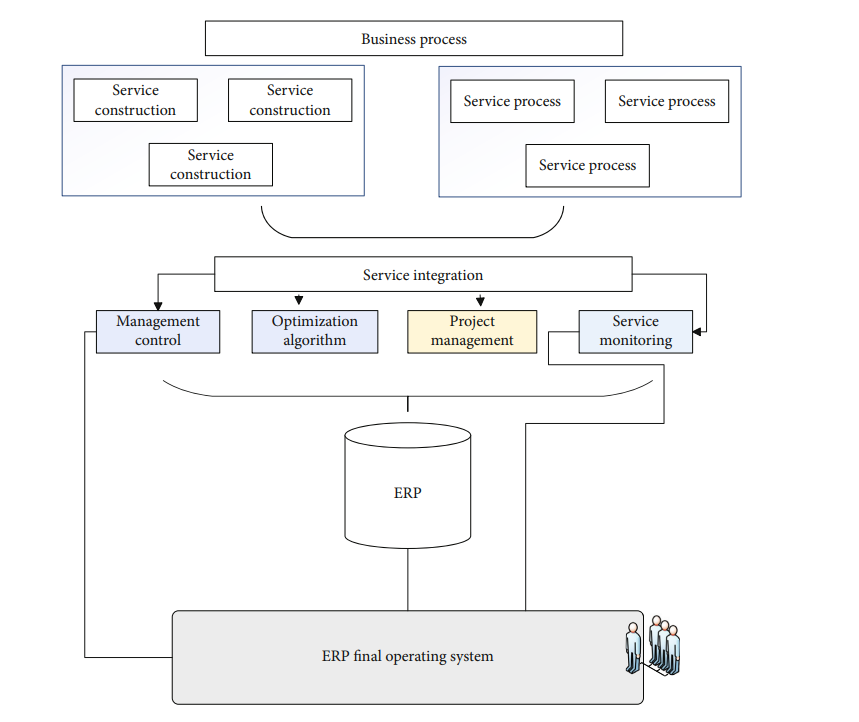
\includegraphics[width=1\linewidth]{img/ERP system framework hierachy.png}
    \caption{ERP System Framework Hierarchy}
    \label{fig:enter-label}
\end{figure}
\par{The diagram shows how an ERP system interprets the defined business process and how it processes this information to generate an effective output. The services that occur during the business process are integrated with a system that monitors, optimizes, and manages these processes and in turn a completed ERP system is created. }
\subsection{Features of ERP Systems}
\par{There are various features that make up an ERP system, however there is no set standard for what an ERP system must be able to functionally do as ERP systems are configured for the need of the company it is built for. However, generally ERP systems can potentially have any of the following features that are discussed and examined below:}
\subsubsection{Financial Management}
\par{The benefits of implementing enterprise systems for accounting have not been thoroughly studied globally. Furthermore, there are surprisingly few studies that thoroughly investigate the connection between ERP user happiness and accounting gains \citep{kanellou2013accounting}. Nonetheless, there are studies concentrating on the relationship involving ERP systems and accounting in the pertinent literature. \cite{spathis2004enterprise} investigated the adjustments taking place in terms of accounting software as well as the factors that led businesses to decide to replace their outdated information systems with fully functional ERP systems. The findings demonstrated that the three primary drivers of ERP adoption were the growing requirement for immediate data, the requirement for integration between applications, and the production of information for decision-making. Greater data production flexibility, increased accounting application integration, better report quality (statement of accounts), better decision-making based on timely and accurate accounting information, and a shorter yearly account closure period were the main accounting benefits of ERP implementation.

It was discovered that ERP systems can support novel accounting procedures and serve as data sources for them. More precisely, ERP systems appear to help with data collecting and the organisational scope of management accounting, according to \cite{rom2006enterprise} This was further supported by \cite{spathis2004enterprise} who pointed out that the use of these systems encourages the adoption of innovative management accounting practices and improves accountants' efficiency in carrying out daily tasks, managing large databases, and producing reports swiftly and adaptably.

\cite{kanellou2013accounting} concluded that there are several advantages to using an ERP in the accounting department, and the most of these are well regarded. Therefore, the case can be made that an organisation should integrate accounting with its ERP system. Lastly, it is noted that there is a positive correlation between ERP cost and ERP advantages and the degree of ERP user satisfaction. These conclusions are very encouraging and as financial management is a lacking feature within the TaskFlow system, the further development of this integral functionality will be made a priority throughout the case study project.}
\subsubsection{Human Resources Management}
\par{Enterprise managers' main concerns in modern times are increasingly intense business competition amongst enterprises and how to draw in the best talent to become part of the workforce, streamline human resources, cut personnel costs, and increase the competitiveness of enterprises; in other words, these enterprise managers believe that the integration of ERP into the HR system has expanded the system's capabilities to encompass enterprise management. The variety of HR services has expanded as well, from payroll accounting and personnel administration to a comprehensive suite of tools that support business decision-making. Planning for human resources, staff appraisal, scheduling, time management, hiring, payroll, training initiatives, and travel administration are some of these topics. They combine to create an effective and highly integrated ERP, together with the financial and production systems \citep{zhao2021research}.

\cite{zhao2021research} proposes a figure showing the impact of ERP systems in increasing the efficiency of HR procedures within a business. The figure can be seen below and proves the worth and effectiveness of implementing this type of system into the HR workforce.}
\begin{figure}[ht!]
    \centering
    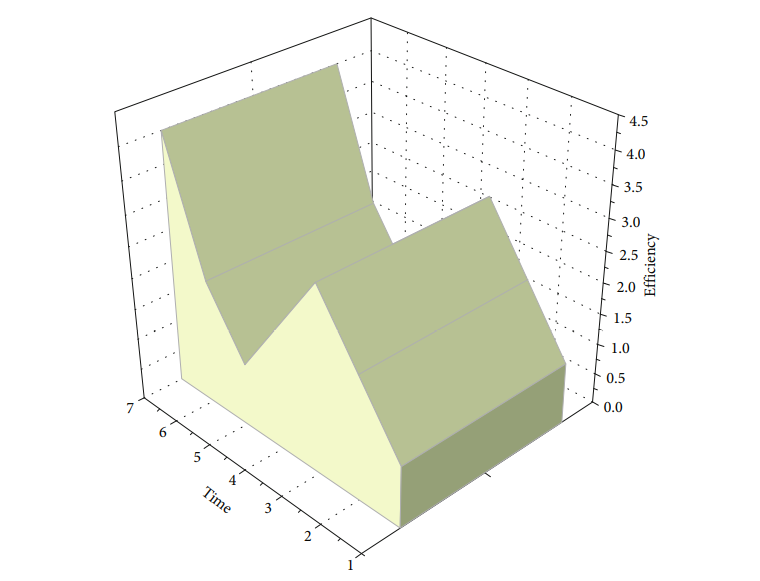
\includegraphics[width=1\linewidth]{img/Human resource management system optimization rate..png}
    \caption{Human resource management system optimization rate}
    \label{fig:enter-label}
\end{figure}
\subsubsection{Supply Chain Management}
\par{The ERP's supply chain component manages all retail operations, including shipments, receipts, issues, and quality control. If you work for a manufacturer, wholesaler, or retailer, managing your inventory is essential to keeping expenses under control and guaranteeing the seamless running of your company. The core functions of every organisation, stock management and valuation, require a significant investment of time and money. Every item's lot-by-lot stock is kept track of, and several computerised information reports are offered to monitor stock movement \citep{ahlawat2017role}.

The ERP supply chain activities include determining the amount of inventory needed, establishing goals, receiving and delivering goods, maintaining materials in stock subsections, categorising every product, supplying materials to the fabrication department, and fully documenting supplier rejections. Additionally, it offers alternatives and strategies for restocking, keeps track of item usage, reconciles inventory balances, and reports the state of inventory \citep{ahlawat2017role}.}
\subsubsection{Customer Relationship Management (CRM)}
\par{The phrase "customer relationship management (CRM)" refers to the capacity to continuously engage with customers across a range of channels; it offers the frameworks necessary for businesses to grow and improve their customer offerings and draw in new ones. Companies are now more interested in knowing their customers and interacting with them in order to seize opportunities and overcome obstacles as a result of the growing rivalry in the business world \citep{kostojohn2011crm}.

Early in the 1990s, CRM was created with the purpose of managing sales teams and direct marketing, as well as preserving consumer data and reaching their preferences from past purchases and conversations \citep{bygstad2013social}. CRM was created to provide a range of essential tools that could be used by businesses of all sizes and in a variety of industries. These tools would enable them to monitor, manage, and share customer data \citep{smilansky2015select}, aid salespeople and marketers in examining the behaviour of their clients, and add value to the company through the use of both human and technological resources \citep{bibiano2014initial}. Therefore, businesses become more competitive, maximise revenues, decrease effort duplication, improve the effectiveness of information storage, make it available to all employees, and provide a single overview to partners and customers. CRM systems comprise the techniques, tools, and capacities that assist an organisation in managing its customer relationship. A significant portion of this work is closely related to the advancement of information and communication technology, which allows businesses to gather the most data possible about their clients' behaviour, contact details, and other characteristics. It also gives them access to efficient tools and methods for managing this data. Thus, the concept of CRM refers to the ability for businesses to better manage their clientele by implementing dependable systems, processes, and procedures that enable them to obtain the most data about their clientele and interact with them for business objectives in order to obtain specific information that aids in the targeting of goods, services, and new markets \citep{ronchi2009eculture}.}
\subsubsection{Inventory Management}
\par{Real-time data on inventory levels and values, encompassing stock on order, raw materials, ongoing work, and completed products, is provided by ERP software. The ERP inventory component handles all aspect of a company's stock-related operations. An inventory management module is a tool that makes collecting information in the inventory department or warehouse quicker and can assist you in keeping the right amount of stock on hand \citep{ahlawat2017role}.

The supply and demand sides benefit from the application of an inventory management methodology. Inventory management can improve the speed of delivery and stabilise interactions with clients for the supply side. On the demand side, it also lessens the impact of inventory on financial resources, lowers the possibility of material deficits, and quickens the supply chain's reaction time \citep{zhao2021research}.

\cite{zhao2021research} proposes two a flow charts that symbolise the functioning of production, inventory, procurement, and the payment process within an ERP system. This example can be further generalised and seen as a general flow chart of how and ERP system technically and practically functions within a given component of the system which in this case is inventory management. Both these flow charts can be studied below:}
\begin{figure}[ht!]
    \centering
    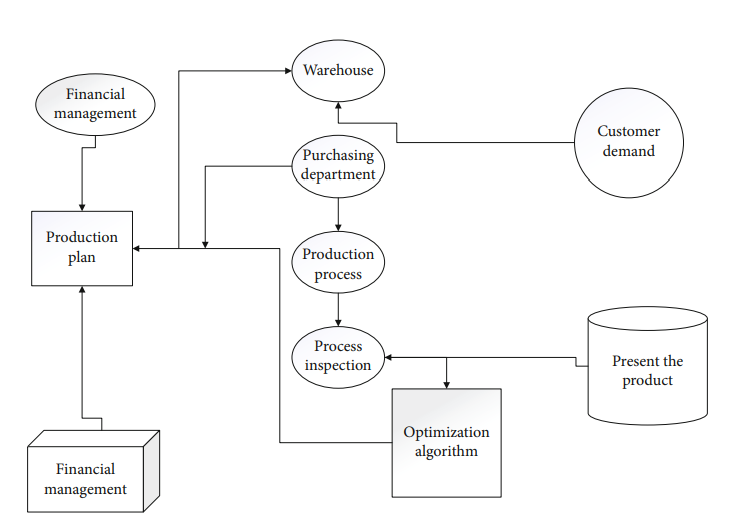
\includegraphics[width=1\linewidth]{img/rename flow chart of company's inventory and production.png}
    \caption{Flow chart of the company’s production and inventory business based on ERP system}
    \label{fig:enter-label}
\end{figure}
\pagebreak
\begin{figure}[ht!]
    \centering
    \includegraphics[width=1\linewidth]{img/Flow chart of the company’s ERP-based procurement and payment process.png}
    \caption{Flow chart of the company’s ERP-based procurement and payment process}
    \label{fig:enter-label}
\end{figure}
\par{Within this basic examples we can see how the business process would hypothetically flow and how data moves to and from a database storing the information necessary to produce some sort of return. This concept can be applied throughout various modules of an ERP system. Each function is always user input that is processed, stored in a database, and then an output that is once again returned to the user.}
\subsubsection{Sales and Marketing}
\par{A system was created as a tool to address particular business functions beginning in 1975 \citep{monk2013concepts}. This technology allows for the automation of business function-related tasks and transactions. Nevertheless, the organization's inter-area business operations must manually transfer data because each system is tailored to a particular business function and there is no system integration. Therefore, the likelihood of data duplication is relatively high. For instance, if the finance and supply chain functions also need data on the sales business function, the data is just being reproduced to meet the requirements. This is the primary justification for using a single database for incorporating part or all of an organization's business processes through enterprise resource planning.

It is anticipated that this technology will enable all organisational transactions to be automated and eliminate the requirement for manual data sharing amongst all business operations. Because of this, having an ERP system in place is crucial to an organization's ability to operate profitably \citep{tsai2008impact}.
    
A business is a company that makes money by selling products or services to customers. Many of the transactions that take place throughout its operation involve businesspeople. The transactions typically comprise a range of organisational data, such as the quantity of inventory, the volume of revenue flowing in and going out, the quantity of goods that need to be produced. Furthermore, transactions typically result in the production of a number of documents, including sales orders, invoices, quotes, and inquiries \citep{xu2008review}.

By making proper use of an ERP system to automate and manage sales and marketing tasks, \cite{terminanto2017implementation} suggests the following improvements can be made:}
\begin{itemize}
    \item Employ an ERP system to save and combine data from all divisions into a single system.
    It is anticipated that divisions will be able to coordinate more effectively with the data recorded in the system.
    \item Generating a quote form through the ERP system. Sales no longer have to access different kinds of papers in order to finish filling out the offer form thanks to the ERP system. Sales can access the system's database and enter the information required to create a quote straight away. Additionally, since the quotation form is automatically prepared and kept in the system, sales do not need to save it in and external system.
\end{itemize}
\subsubsection{Business Intelligence (BI)}
\par{Business Intelligence (BI) solutions are becoming the centre of attention for companies when it comes to information systems. The advantages of business intelligence (BI) differ greatly amongst companies. Due to their ability to combine, integrate, and analyse the massive volumes of transactional data produced by ERP systems, business intelligence (BI) solutions are increasingly utilised as extensions of ERP systems \citep{hawking2010business}.

New apps and the growth of current IT systems were brought about by the need for better information analysis as well as advancements in related technologies.
Collaborative systems (CS), corporate performance management (CPM), analytics, knowledge discovery (KD), data mining (DM), and knowledge management (KM) were among them. All of the above listed systems are now frequently referred to as business intelligence (BI) \citep{gibson2004evaluating,olszak2007approach}.

In today's corporate environment, business intelligence (BI) is deemed highly priority by many firms due to its potential to significantly impact their performance. Companies who employ business intelligence (BI) properly can generate an average return on investment (ROI) of 401 percent over a three-year period, according to \cite{power1998justifying}. 70 percent of the 142 organisations surveyed by \cite{herzum2003cutter} reported that they were putting data warehousing and business intelligence efforts into practice. Leading business analyst firm \cite{gartner2009gartner} polled 1,500 Chief Information Officers globally and determined that business intelligence (BI) was the most important technology priority. Accordingly, it is predicted that by 2012, revenue from BI vendors will amount to 7.7 billion dollars \citep{sommer2008gartner}.}
\subsection{Competition within the ERP System Industry}
\par{The biggest players within the ERP space are SAP, Oracle, and Microsoft. These companies provide the software solutions for business process management on the largest scale. These companies are direct competitors for one another but have less impact on small and medium sized companies who rather go for more affordable and practical solutions. Within the South African space, these small and medium companies make use of Monday.com, Zoho, SalesForce, Clickup, and similar software such as what is being built and sold at Taskflow. This section will proceed to review and compare these various providers and their commercialised systems to determine what commonality there is between them and identify the base requirements of a fully functional ERP system.}
\subsubsection{SAP}
\par{In 1972, Hopp, Wellenreuther, Hector, Plattner, and Tschira developed the SAP method \citep{o2015sap}. The SAP method is made up of a number of fully integrated components that cover almost every aspect of a professional organisation. The SAP approach is the primary source of supply for the ERP system keys industry. In 2012, the SAP software system held around 25 percent of the market and industry.However, Oracle software came in second with 13 percent of the market share, followed by Microsoft Dynamics with 5 percent. SAP is a very large company that does not focus exclusively on its most lucrative ventures. Their produce is truly minor commercially approachable, catering to hundreds of customers who make up less than 1,000 society members. 

When one learns the fundamentals of the SAP software system, it becomes a simple tool to utilise even though it may take some time for individuals unfamiliar with it to make the switch from Microsoft Dynamics and Oracle. SAP software systems tend to be more expensive than their competitors, even though prices can vary depending on features and benefits. This makes them less than ideal for small to medium-sized businesses with limited IT funding \citep{annamalai2011enterprise}.}
\subsubsection{Oracle}
\par{Oracle software E-Business Collection \citep{barr2014oracle} is a potent ERP programme with a wide range of features and advantages that have helped elevate it to the status of one of the most advanced ERP programmes available today. For ease of use, Oracle software system E-Business Group may smoothly merge several components into a single system. Additionally, Oracle E-Business Group enables users to automate a number of processes, eliminating the need for human data entry. In addition to increasing efficiency and productivity, this also fixes errors and guarantees that data is not lost. 

The Oracle software system E-Business Collection has the ability to record the course of inventory levels at Business Company. Should an item's inventory level drop beneath a predetermined positive standard, the system will immediately provide purchase orders. Very powerful, durable, and intuitive ERP software is the Oracle software system EBusiness Collection, which can meet the needs of almost any industry. Businesses build their own individual elements since the predefined tax element and sales units on the Oracle E-Business Group are frequently insufficient \citep{barr2014oracle}.}
\subsubsection{Microsoft}
\par{Microsoft Dynamics Marketing is built on Microsoft infrastructure, as its name implies. It synchronises and develops flawlessly with additional Windows commercial requests, facilitating the effortless distribution of data across all methods organisations. Microsoft Dynamics synchronises with various Windows applications, as previously mentioned, simplifying data sharing and transfer. It is built on a Windows substructure and takes a lot less time to implement Microsoft Dynamics Marketing than other approaches. takes the least amount of time to apply out of the three, according to Panorama Consulting Solutions \citep{solutions2016report}. Large, international industries find Microsoft Dynamics ideal as it supports multiple languages and can work with a variety of currencies in close proximity to global marketing.}
\par{\cite{mayer2017clash} proposes the table below to draw comparisons between these three ERP systems:}
\begin{table}[ht]
    \centering
    \scriptsize
    \begin{tabular}{|l|c|c|c|}
    \hline
    & \textbf{SAP} & \textbf{Oracle} & \textbf{Microsoft Dynamics} \\ \hline
    Store Part & 19\% & 13\% & 16\% \\ \hline
    Short-list Rate & 38\% & 18\% & 31\% \\ \hline
    Collection Rate When Short Recorded & 38\% & 22\% & 22\% \\ \hline
    Application Period & 23.1 months & 24.5 months & 23.6 months \\ \hline
    Total Price of Ownership & \$2.09 million & \$2.38 million & \$2.06 million \\ \hline
    Reimbursement Period & 30 months & 29 months & 12 months \\ \hline
    Disruption at Go-live & 44\% & 42\% & 41\% \\ \hline
    Realised 50\%+ of Anticipated Business Benefits & 34\% & 21\% & 26\% \\ \hline
    \end{tabular}
    \caption{Comparison of SAP vs. Oracle vs. Microsoft Dynamics}
\end{table}
\par{The table shows that all three of these systems perform similarly across the measurement categories, however it seems SAP remains the most popular and sits in the middle of the three systems when it comes down to cost of ownership and is the most successful in terms of realising the anticipated benefits of system implementation.}
\subsubsection{Monday.com, Zoho, and Taskflow}
\par{These are the three relevant systems when it comes to the ERP system in South Africa. While there are other competitors such as ClickUp, not all available systems will be reviewed in this research paper as there are large amounts of ERP systems available and the lines between what is classified as ERP and what is not have become blurred, therefore it is only necessary to review these three systems. As SAP, Oracle, and Microsoft have overpowered the industry in terms of landing large corporations as clients, these three systems and many others aim to fulfill the needs of small and medium-sized businesses. In this subsection the function of these three systems will be outlined and then compared to review the differences.

Monday.com is a cloud-based work operating system that enables groups to design workflow applications for managing daily tasks, projects, and procedures. For organising, monitoring, and controlling tasks and projects, it offers a versatile and graphical platform. Customisable workflows, task management, team collaboration tools, and interfaces with several third-party apps are some key features. By providing communication, file sharing, and reporting capabilities in one location, it is intended to increase efficiency and simplify project administration \citep{monday.com}.

Zoho is a comprehensive suite of cloud-based business applications designed to help organisations manage various aspects of their operations. It includes tools for customer relationship management (CRM), finance, human resources, project management, email, and collaboration. Zoho's products are known for their integration capabilities, allowing businesses to streamline processes and improve efficiency. The platform is widely used by small to medium-sized enterprises for its affordability, scalability, and extensive range of features \citep{zoho}.

Taskflow is a software platform designed to manage and automate workflows and tasks within an organisation. It provides tools for task management, project tracking, and process automation, enabling teams to collaborate efficiently and stay organised. Taskflow typically includes features like customisable workflows, task assignments, deadline tracking, and reporting. It is designed to adapt to various business needs, helping improve productivity and streamline operations by ensuring that tasks are completed in a structured and timely manner \citep{taskflow}. The table below compares these various systems.}
\begin{table}[h!]
    \centering
    \resizebox{\textwidth}{!}{
    \begin{tabular}{|l|l|l|l|}
    \hline
    \textbf{System} & \textbf{Monday.com} & \textbf{Zoho} & \textbf{TaskFlow} \\ 
    \hline
    \textbf{Core Functionality} & 
    \begin{tabular}{l}
    - Task and project management \\
    - Customisable workflows \\
    - Team collaboration tools \\
    - Integrations with third-party apps
    \end{tabular} & 
    \begin{tabular}{l}
    - Customer relationship management (CRM) \\
    - Finance management \\
    - Human resources \\
    - Project management \\
    - Email and collaboration tools
    \end{tabular} & 
    \begin{tabular}{l}
    - Task management \\
    - Project tracking \\
    - Process automation \\
    - Customisable workflows \\
    - Reporting
    \end{tabular} \\
    \hline
    \textbf{Pricing} & 
    \begin{tabular}{l}
    - Varies based on plan: Basic, Standard, Pro, Enterprise \\
    - Starting at around \$8/user/month
    \end{tabular} & 
    \begin{tabular}{l}
    - Varies widely depending on products chosen \\
    - Free and paid tiers \\
    - Zoho One: \$37/user/month for the full suite
    \end{tabular} & 
    \begin{tabular}{l}
    - Custom pricing based on business needs \\
    - Typically enterprise-level pricing
    \end{tabular} \\
    \hline
    \textbf{Attributes} & 
    \begin{tabular}{l}
    - Visual and user-friendly interface \\
    - Highly Customisable \\
    - Suitable for teams of all sizes \\
    - Strong integration ecosystem
    \end{tabular} & 
    \begin{tabular}{l}
    - Comprehensive suite of business applications \\
    - Scalable for small to medium-sized businesses \\
    - Strong focus on affordability and integration \\
    - Extensive range of features
    \end{tabular} & 
    \begin{tabular}{l}
    - Designed for workflow automation \\
    - Adaptable to various business needs \\
    - Focused on improving productivity and task management \\
    - Enterprise-level customization and support
    \end{tabular} \\
    \hline
    \end{tabular}
    }
    \caption{Comparison of Monday.com, Zoho, and Taskflow}
\end{table}
\par{The data in the table displays that these systems catering more towards small and medium sized businesses have each found their own business model and sales strategy to increase engagement in their target market as each of these three systems cater for a different audience and have different core functionality.}
\subsection{Components of Developing an Industry Approved Software System}
\par{This subsection and the one that follows will both review the process of creating and implementing an industry approved software system as well as an industry approved ERP system. These subsections will review the standard components of an industry systems development lifecycle and will make reference to the standards and practices that need to be upheld in order for these systems to be successful within the climate of the software development industry, not only in the South Africa, but also the rest of the world.}
\subsubsection{Requirements}
\par{Gathering, examining, and recording stakeholder demands and limitations is the process of requirements analysis, which makes sure the software system satisfies their needs \citep{doe2011recommended}. Since it establishes the framework for all upcoming development efforts, this stage is crucial. Both functional and non-functional requirements—which specify how the system should operate, such as scalability and reliability—should be included in effective requirements documentation \citep{sommerville2011software}.}
\subsubsection{Systems Design}
\par{A blueprint for building the software system is created by system designers using requirements. Determining the \citep{jacobson2021unified}. Good design makes sure that the system's structure satisfies its needs and is efficient, scalable, and maintainable.}
\subsubsection{Implementation}
\par{Developing the program in accordance with the design standards is part of implementation. During this stage, code is written, reviewed, and integrated to make sure it complies with quality standards and design criteria. Maintaining code quality requires adhering to best practices in coding, which include employing version control and coding standards \cite{mcconnell2004code}.}
\subsubsection{Testing}
\par{Testing confirms that the programme satisfies all requirements and functions as planned. It includes a variety of testing techniques, including system testing (evaluating the complete system), integration testing (examining how components interact), and unit testing (evaluating individual elements) \citep{istqb2011foundation}. Finding and fixing issues before release is the main objective \citep{myers2011art}.}
\subsubsection{Quality Assurance}
\par{Planned actions are taken as part of quality assurance (QA) to guarantee that software fulfils quality standards at every stage of development \citep{team2002capability}. This include creating quality measures, carrying out evaluations, and putting procedures in place to raise the standard of quality. QA seeks to stop errors and guarantee dependable and effective software \citep{international2011systems}.}
\subsubsection{Deployment}
\par{Software must be released into the production environment in order for deployment to take place. This stage involves setting up the program, installing it, and making sure it runs properly in a live environment. Thorough preparation is necessary for a successful deployment in order to reduce disruptions and guarantee a seamless transition for users \citep{sommerville2011software}.}
\subsubsection{Maintenance}
\par{Software systems need to be updated and fixed on a regular basis after they are deployed. To guarantee that the program continues to satisfy the requirements of users and runs safely and effectively, maintenance entails correcting, adaptive, and preventative actions \citep{pressman2005software}. An essential component of the maintenance stage is managing patches and version updates.}
\subsubsection{Security}
\par{To protect the system from weaknesses, security is incorporated across the whole lifetime. According to \cite{goodrich2011introduction}, these include of restricted access, the use of encryption, secure programming techniques, and frequent inspections of security. To make sure the infrastructure is resistant to threats, penetration tests and vulnerability inspection are helpful.}
\subsubsection{Documentation}
\par{Regarding both current development and upcoming upgrades, comprehensive documentation is crucial. This includes system architecture, code, user manuals, and maintenance procedures \citep{doe2011recommended}. By acting as a communication mechanism between stakeholders, documentation guarantees the maintainability and understandability of the system.}
\subsubsection{Compliance}
\par{According to \cite{sommerville2011software}, compliance is the system's conformity to legal, regulatory, and industry standards including SOX, GDPR, and HIPAA. Compliance guarantees that the system complies with legal requirements for data security, privacy, and operational openness.}
\subsection{Components of Developing an Industry Approved ERP System}
\par{This subsection will once again review the same components as before, except making specific reference to ERP systems, how they differ from other system implementation within the software industry, and providing detail into actions within the process that result in a successful systems development process.}
\subsubsection{Requirements}
\par{Due to the cross-functional nature of ERP systems—which integrate numerous business processes—gathering requirements is one of the most important stages of the process. ERP systems must take into account the needs of different divisions, notably supply chain, customer relationship management (CRM), finance, and human resources, as opposed to normal software projects. ERP failure can result from incorrect or poorly stated requirements, which is concerning considering the high expense and complexity associated with ERP implementations \citep{monk2013concepts}. The requirements gathering process, which makes sure the ERP system will fulfil organisational goals, consists of several steps, including discovery, stakeholder interviews, and business process modelling \citep{esteves2001enterprise}. }
\subsubsection{Systems Design}
\par{According to \cite{monk2013concepts}, ERP systems are made to be modular, enabling businesses to implement just the elements they need to run the system without compromising its integrity. While one module must fluidly interface with the others, system design is made more complex by this modularity. The financial module of an ERP system, for instance, needs to interface with the modules for inventory, procurement, and manufacturing in order to guarantee correct financial reporting. Scalability is another important consideration in system design because enterprise environments typically have high transaction and user volumes \citep{o2000enterprise}. The ERP software that is selected has a significant impact on the design phase. Programs like SAP, Oracle ERP, or Microsoft Dynamics have predefined workflows and data structures that need to be customised to meet the unique requirements of the company. The incorporation of external systems, such as customer relationship management (CRM) software and business intelligence (BI) platforms, should also be taken into account throughout the design phase as it is common practice create intergrations between different platforms due to client requirements.}
\subsubsection{Implementation}
\par{The process of implementing an ERP involves several stages, including configuration, training, data migration, and customisation. According to \cite{zhang2003critical}, customisation usually refers to changing ERP modules to satisfy certain business demands, including special processes or regulatory constraints. Contrarily, configuration entails adjusting the ERP system's parameters—like tax rates or payment terms—to match the operational framework of the company. Data migration, or moving data from old systems into the ERP, is one of the trickiest parts of implementing an ERP. Due to data inconsistencies, missing data, or variations in data architecture, this might get complicated. To reduce disruption, ERP systems usually take a staged approach, rolling out modules one at a time \citep{shanks2000model}. }
\subsubsection{Testing}
\par{According to \cite{ahmad2013critical}, testing in ERP systems is more complicated than testing in traditional software since ERP connects several business processes from different departments. Integration testing examines the interactions between these modules, whereas functional testing verifies that each module—for example, finance, HR, and procurement—functions as intended. For instance, adjustments to inventory levels ought to be automatically reflected in the finance module. Because it involves end users running real-world scenarios, user acceptability testing (UAT) is essential to verifying that the system satisfies business needs \citep{nah2001critical}. Furthermore, especially in international organisations, performance testing is essential to guarantee that the system can manage large numbers of users and transactions. To safeguard critical data, like payroll data and financial records, ERP testing should also involve security testing.}
\subsubsection{Quality Assurance}
\par{ERP systems use quality assurance (QA) to make sure the solution satisfies technical and business objectives and is error-free \citep{hawari2010explaining}. QA is a multi-layered process that begins with automated testing and code reviews to identify problems early in the development cycle. Validating that business processes match the ERP configuration and that workflows and transactions flow correctly between modules is another aspect of quality assurance (QA) in ERP installations. Due to the significant financial and operational risks connected with defects—which could lead to erroneous financial reporting, disruptions in the supply chain, or non-compliance with regulations—quality assurance (QA) is crucial for ERP systems \citep{hawking2004revisiting}. ERP providers frequently offer QA-specific solutions, like SAP's Solution Manager, which aids businesses in managing their QA procedures.}
\subsubsection{Deployment}
\par{ERP deployment is usually carried out in stages to reduce business impact. This usually entails introducing one department or module at a time, beginning with less important tasks and working your way up to more crucial ones like supply chain management or finance \citep{monk2013concepts}. While more risky, "big bang" deployment strategies—where the entire system goes online at once—are occasionally chosen by businesses that need to make urgent system-wide modifications. Because they provide more flexibility, quicker deployment periods, and lower infrastructure costs than conventional on-premise systems, cloud-based ERP systems—like Oracle ERP Cloud or SAP S/4HANA Cloud—are becoming more and more popular \citep{vukovic2023erp}. Cloud-based ERP systems, however, could run into issues with data security, compliance, and limited customisation options.}
\subsubsection{Maintenance}
\par{After going online, maintaining the ERP system becomes a constant effort that involves routine upgrades, bug patches, performance enhancements, and modifications to accommodate evolving corporate needs \citep{ahmad2013critical}. Patches and upgrades are routinely released by ERP suppliers; these must be tested and implemented without interfering with regular business operations. Updating the system to account for new business procedures or regulatory changes—like entering new markets—is another aspect of maintenance. Maintaining ERP effectiveness is essential to keeping the system in line with the changing needs of the company. Reduced ROI, elevated security threats, and operational inefficiencies might result from improper ERP system maintenance \citep{hawking2004revisiting}.}
\subsubsection{Security}
\par{ERP systems manage enormous volumes of sensitive data, including personnel records and financial data, thus security is a top priority. Access controls, encryption, and frequent audits are only a few of the layers that make up ERP system security \citep{tarafdar2003analyzing}. ERP systems frequently employ role-based access control (RBAC) to make sure that users can only access information and take actions that are appropriate for their position. ERP providers help businesses manage risks and maintain regulatory compliance by offering integrated security capabilities, such as SAP's Governance, Risk, and Compliance (GRC) solutions \citep{hawari2010explaining}. To find possible threats and reduce risks, regular penetration tests and vulnerability assessments are crucial.}

\section{Implementation of ERP Systems}
\par{The seven main steps in the ERP deployment process include business process analysis, software installation, data migration, software performance testing, user training, complete deployment, and post-implementation support \citep{ly2020definitive}. These main key steps are examined in greater depth in the sections that follow.}
\subsubsection{Business Process Research and Requirements Gathering}
\par{The first step in the ERP implementation procedure is to define the needs, goals, and scope of the ERP within the specified business' process. Building a team that can work on the ERP implementation project from beginning to end is also necessary \citep{wetherbe2006information}. Within the team there would mainly be two roles, software developers and the sub roles that preside within this overarching role, as well as business analysts that are responsible for documenting and understanding the business process and how it will be converted into an ERP system. This step within the implementation process is largely the responsibility of the business analysts. The responsibilities of the business analyst within this step of the process would be as follows \citep{yusuf2004enterprise}:}
\begin{itemize}
    \item Analyse, record, and describe an organisation's current procedures. 
    \item Look for significant difficulties, process waste, and customer-focused problems.
    \item Establish clear objectives for an ERP deployment that are connected to the major success areas, and quantify them precisely.
    \item Create a cost budget and a solid timetable.
\end{itemize}
\subsubsection{Software Installation}
\par{Following the first step's creation of new procedure flows, the team should have a new business process plan in place. The architecture and infrastructure for software, such as the data store, data presentation, and internet accessibility, will be installed and constructed by the software developers who have recieved the business requirements from the business analyst.}
\subsubsection{Data Migration}
\par{In this stage, all data is transferred to a new software platform. Before the data is transferred to a new site, it should all be reviewed and adjusted to ensure a smooth mapping process. Data mapping between the previous and new store locations, data transfer, and the configuration of a new data storage location are all included in this stage.}
\subsubsection{User Training}
\par{Personnel react to change management, and user training relies on the intricate nature of the ERP program. Up to 56 percent of ERP deployment cases after go live result in production halts under training.}
\subsubsection{Final Deployment}
\par{Depending on the scale of the ERP software and the assets available, the organisation might select one of the following three ways:}
\begin{itemize}
    \item Big-Bang Method: A one-day switch from the outdated to the updated software. This method is quick and inexpensive, but any inefficiency in deployment could lead to a serious issue during use.
    \item Phased Approach: A longer-term, function- or unit-specific phased transition.
    \item Parallel Operation Approach: In order to reduce risk, users use both new and old systems simultaneously.
    This method has greater operational expenses for the two platforms and necessitates more time for repetition of work.
\end{itemize}
\subsubsection{Support}
\par{Performance review of ERP projects is crucial and should be done for the duration of the project. Key performance indicators that can be compared are as follows:}
\begin{itemize}
    \item Real implementation costs compared to the budgeted amount
    \item The return on investment for the project
    \item The assessment of mistakes or human errors
    \item The efficiency of the supply chain and production
    \item The satisfaction of customers and their willingness to continue working with the development company
\end{itemize}
\subsection{ERP Implementation Time}
\par{Once the software system is launched, an ERP system implementation project may take anywhere from three months to several years to complete and fully implement to a point where both client and development company are satisfied \citep{sankar2006implementation}. The size of the organisation, the volume of data, the number of users, and the resources all affect how long the ultimate project implementation takes \citep{pelphrey2015directing}.}

\section{Critical Competencies for Software Development}

\section{The Information Technology Industry}
\subsection{Challenges within the Information Technology Industry}
\subsection{Challenges Exclusive to Developing Nations}
\subsubsection{The Purpose of a University}
\subsection{Developing Nations vs. The Rest of the World}

\section{The Value Chain}
\subsection{People}
\subsection{Processes}
\subsection{Technology}
\subsubsection{Hardware}
\subsubsection{Software}
\subsubsection{Infrastructure}
\subsection{The Economic Viability of Academic and Industry Partnership}
\subsection{Industry Offering Resources to Universities}

\section{Commercialization of Software}
\subsection{Methods of Commercialization}
\subsubsection{Recommendation}

\section{Students in Industry}
\subsection{Advantages}
\subsection{Threats}
\subsection{Similar Projects}

\section{Project Management Methodologies}
\subsection{Software Development Management Methodologies}
\subsection{Recommendations}

\section{Artefact}
\subsection{Methods for Measuring Artefact Success}
\subsection{Methods for Measuring Artefact Functionality}
\subsection{TAM Model}